% Generated from 20-企业分析框架.md; edit the LaTeX source after migration.

\reportpart{第二十部分 企业分析框架}
\addcontentsline{toc}{part}{第二十部分 企业分析框架}
\markboth{第二十部分 企业分析框架}{第二十部分 企业分析框架}

在具身智能领域，企业信息极易沦为新闻流和 demo 流。如果没有统一分析模板，就很容易被融资额、宣传片和单次演示带偏，而忽略真正决定长期价值的技术与交付变量。因此，本部分的职责，是先建立一个稳定的企业分析框架，再在后文具体公司章节中重复使用。

这一框架的必要性在 2024-2026 年尤为突出。Figure、Physical Intelligence、Apptronik、Agility、1X、Sanctuary AI、特斯拉 Optimus、优必选、宇树、智元等公司分别站在“通用本体”“VLA/基础模型”“工业交付”“物流场景”“人形平台”“远程接管”和“中国制造链协同”等不同位置上。若没有统一模板，很容易把风格完全不同的公司放在同一维度上比较，最后只剩下谁更会讲故事、谁视频更好看，而看不见底层变量。相关公司主页可参见 \href{https://www.figure.ai/}{Figure 官网}、\href{https://www.physicalintelligence.company/}{Physical Intelligence 官网}、\href{https://agilityrobotics.com/}{Agility Robotics 官网} 与 \href{https://www.ubtrobot.com/}{优必选官网}。

更进一步说，企业分析框架的真正意义不是“做成一张表”，而是把企业研究从新闻消费转成结构化判断。报告后续任何一版更新，只要能坚持使用同一套问题集，就能够积累跨时间、跨公司、跨路线的比较能力，而不是每次都重新被新的品牌叙事带走。

\section*{95. 为什么企业需要统一分析模板}
\addcontentsline{toc}{chapter}{95. 为什么企业需要统一分析模板}
\markboth{95. 为什么企业需要统一分析模板}{95. 为什么企业需要统一分析模板}

\subsection*{95.1 防止沦为新闻罗列}
\addcontentsline{toc}{section}{95.1 防止沦为新闻罗列}


企业分析最常见的失效方式，就是把连续发生的融资、发布会、合作新闻和 demo 视频顺次堆进报告，最后得到一份“信息很多但判断很弱”的时间流。之所以需要专门强调这一点，是因为具身行业本身就处在高波动、高叙事密度阶段，如果没有稳定框架，研究者很容易在更新过程中被最新事件牵着走，而丢失对企业长期能力结构的判断。

更稳健的做法，是把任何新增新闻都强制回写到既定分析维度中，例如它究竟改变了数据获取、系统集成、制造交付、客户进入还是资本耐心。只有当事件真正改变其中某一条能力链条时，它才值得进入正文判断；否则，它更适合作为跟踪日志而不是结构性结论。这个规则看似保守，但正是防止企业章节退化成“资讯摘要”的关键。 企业分析框架首先要解决的，就是避免把研究写成“按时间顺序堆新闻”。新闻罗列最大的问题不只是冗长，而是它会把高频曝光误当作高价值进展，把单次演示误当作能力跃迁。一个稳定框架的意义，在于无论企业发了多少视频、融资稿和发布会材料，我们都始终用同一组问题去过滤信息。

更具体地说，每条企业信息至少都应被追问三件事：它说明的是能力、接口、落地还是资本信号；它是一次性展示还是可重复趋势；它对应的证据强度来自论文、开源、客户部署还是市场宣传。只有把这三层拆开，企业研究才不会被节奏带着走。 企业分析之所以极易滑向新闻罗列，是因为外部公开信息天然偏向“融资、合作、发布、演示”这些传播友好事件，而真正决定公司位置的底层变量反而更难直接被看见，例如数据闭环是否真实建立、现场部署是否持续、失败恢复是否被系统性吸收、供应链是否开始收敛。统一模板的价值，就在于强迫分析从传播事件退回到系统变量，而不是被舆论节奏牵着走。

没有统一框架，企业章节往往会退化为时间线式材料堆叠，难以横向比较。

因此，这一章最重要的产出并不是“这次列了哪些公司”，而是留下了一套之后每个季度都能继续用的问题集。后续企业更新若偏离这套问题集，章节质量就会迅速回落到新闻摘要层。

\subsection*{95.2 便于横向比较}
\addcontentsline{toc}{section}{95.2 便于横向比较}


横向比较的目标，不是给所有企业排一个简单名次，而是让它们在相同问题集下暴露各自真正强、真正弱的环节。具身领域里最常见的阅读错觉，是把基础模型平台、本体制造商、场景集成商、共享自治服务商和综合型人形公司直接并排讨论，最后只剩下“谁故事更大、谁视频更好看”。这样的写法看似覆盖很广，实际上并没有形成可复核的判断，因为这些公司解决的根本不是同一层问题。

因此，真正可用的横向比较要先做两步。第一步是“按角色分组”，即先判断一家公司的主销售对象究竟是什么：它是在卖模型接口能力、本体能力、数据闭环能力、场景交付能力，还是制造与运维组织能力。第二步才是“在共同维度上投影”。我更建议固定八个维度：团队背景、技术路线、数据与模型、本体与系统能力、目标场景、商业路径、资本与合作、风险与局限。这样做的意义，不是消除差异，而是把差异压回可以解释的位置。

若把单家公司写成一个粗向量，可以记作：

\begin{equation*}
\mathbf{v}_{\text{firm}} = [T, R, D, B, S, C, F, K],
\end{equation*}

其中，\(T\) 对应团队与组织背景，\(R\) 对应路线角色定位，\(D\) 对应数据与模型闭环，\(B\) 对应本体与系统能力，\(S\) 对应目标场景与任务单元，\(C\) 对应商业路径，\(F\) 对应资本与合作网络，\(K\) 对应关键风险。这个向量的意义不是为了精确算分，而是为了确保后续任何一家企业都必须回答同一组问题。只要问题集稳定，企业章节就不会因为公司叙事风格不同而失去可比性。

同一分析模板真正强制我们反复追问的是：它的主任务单元是什么，它的控制权掌握在哪一层，它的数据与失败回流是否成环，它能否把能力复制到客户现场。只有这些问题被同一口径回答，企业比较才不会退化成传播比较。

目前这套模板已经落成表格版本，见 20-企业统一分析模板。后续版本若要做季度更新，可直接配合 20-企业季度跟踪表模板 使用，把横向比较进一步转成可追踪字段。

\subsection*{95.3 便于后续版本更新}
\addcontentsline{toc}{section}{95.3 便于后续版本更新}


企业分析框架若不能服务后续版本更新，它就只是一份一次性阅读提纲，而不是长期研究工具。一个合格的模板，必须让我们在数月后面对新增论文、融资、客户、事故、合作与产品发布时，能够把新信息直接插回既有维度，而不是整章重写。换句话说，模板的价值不仅在于当下读起来整齐，更在于未来是否支持增量维护。

这要求框架把“长期稳定维度”和“短期变动信号”明确分开。前者包括技术路线、本体形态、主要场景、组织出身和商业模式；后者包括新版本模型、客户试点、季度融资、关键人变动与新演示。只有把两类信息分层存放，后续版本才可能回答三个更重要的问题：哪些事实变了，哪些判断没变，哪些判断需要修正。

因此，本章模板本质上也是版本控制模板。它让企业研究从“每次重写一篇简介”转成“沿同一问题集持续积累判断”。这对本项目尤其关键，因为后续企业章节数量会持续增长，若没有稳定模板，整书很快会被新资讯冲散结构。 企业章节还必须服务于后续版本维护。一个好的结构不是只对当前阅读顺手，而是能在几个月后行业变化时，快速把新增论文、产品、客户、融资和事故插回原有框架中，而不必整章重写。

也就是说，企业框架不仅是阅读工具，还是版本化维护工具。它要求我们把“长期稳定维度”和“短期变化信号”分开放置：前者例如技术路线、本体形态、主要场景；后者例如最新产品发布、合作进展、融资事件和关键人才变动。 从版本维护角度看，这一点尤其关键。只要模板稳定，后续更新就可以把“哪些事实变了、哪些判断没变、哪些判断需要修正”分开记录，而不是每次新开一轮研究都把企业重新写成一篇简介。这使报告能够逐渐积累一种跨时间的判断连续性，而不是不断被新一轮宣传材料刷新记忆。

有模板，后续版本就能按相同结构增量更新，而不是每次重写企业画像。从版本维护角度看，企业分析框架也是报告长期可更新性的关键支点。它允许后续版本只替换“事实层”和“判断层”中的局部内容，而保留相同问题集，从而实现跨版本对照。

\section*{96. 企业统一分析维度}
\addcontentsline{toc}{chapter}{96. 企业统一分析维度}
\markboth{96. 企业统一分析维度}{96. 企业统一分析维度}

\subsection*{96.1 团队背景}
\addcontentsline{toc}{section}{96.1 团队背景}


团队背景之所以应被列为第一层，不是因为创始人履历天然决定成败，而是因为它往往提前暴露了公司最可能形成优势和最可能忽视的问题。来自自动驾驶、控制和机器人学背景的团队，通常更重系统安全、闭环与工程纪律；来自大模型或互联网 AI 背景的团队，往往更擅长统一接口、数据组织和平台叙事；来自制造或工业自动化背景的团队，则更可能在交付、成本和现场适配上走得更稳。

因此，阅读团队背景时最不该做的，是停留在“名校、名企、明星履历”的表层印象。真正值得追问的是：这支团队过去成功解决过哪一类复杂问题；它的知识结构是否覆盖了本体、数据、模型、部署与交付之间的关键断点；以及它是否存在明显的结构性盲区。例如强模型团队是否低估硬件与现场维护，强本体团队是否低估数据工程与持续学习。这些问题比头衔本身更接近企业未来路径。 团队背景不应只写创始人履历，而应回答“这家公司最初是从什么能力起家的”。控制、自动驾驶、计算机视觉、硬件制造、工业自动化、云平台或消费电子出身，会直接影响其早期技术路径、数据获取方式和商业切入点。

一个实用的读法是：团队背景往往不是花边信息，而是企业早期能力边界的线索。例如自动驾驶背景更容易延伸到感知栈和数据闭环，工业自动化背景更容易延伸到场景集成与客户交付，消费电子背景则更可能在成本工程和量产链条上占优。 团队背景之所以重要，不是为了满足公司介绍的完整性，而是因为它往往预示了路线的初始偏置。来自自动驾驶、工业自动化、消费电子、通用大模型、学术实验室或互联网平台的团队，会天然带着不同的问题拆解方式、风险偏好和工程优先级。理解这个出发点，往往能更早解释公司为何强调某类能力、忽略某类约束，以及其后续能否顺利跨越原有能力圈。

看创始人与核心团队是来自学术、工业自动化、自动驾驶、大模型公司还是消费电子，这往往会直接影响其技术与产品路径。

这一维度的重要性还在于，它通常能解释企业为何会优先解决某些问题、忽略另一些问题。团队背景不是花边信息，而往往是路线偏置最早也最稳定的来源之一。

\subsection*{96.2 技术路线}
\addcontentsline{toc}{section}{96.2 技术路线}


技术路线这一项的核心，不是给公司贴上“做 VLA”“做人形”“做世界模型”之类标签，而是判断它把哪一层能力当作主抓手。表面上许多公司都在讲“通用具身智能”，但真正决定路线分化的，往往是它把上限押在模型接口、本体平台、数据闭环、场景交付还是基础设施供给中的哪一环。若这一点不拆开，所谓路线比较就会退化成热词比较。

因此，技术路线分析至少要回答四个问题。第一，公司把系统上限主要押在哪一层。第二，这条路线最依赖什么稀缺资源，例如高质量遥操作、多机真数据、端侧算力、特定本体，还是高约束场景。第三，它的动作接口是什么，是连续控制、action chunk、技能 token，还是显式任务图。第四，一旦关键前提不成立，这条路线最可能以什么方式失效。只有把“主抓手-依赖条件-接口形态-失败模式”一起写出来，技术分析才真正具备判断力。

若把企业路线形式化地压缩，可以记为：

\begingroup
\scriptsize
\begin{equation*}
\mathcal{R}_{\text{firm}} = \bigl(L_{\text{primary}}, I_{\text{action}}, D_{\text{source}}, B_{\text{bottleneck}}\bigr)
\end{equation*}
\endgroup

其中，\(L_{\text{primary}}\) 表示主要押注层级，\(I_{\text{action}}\) 表示动作与控制接口，\(D_{\text{source}}\) 表示核心数据来源，\(B_{\text{bottleneck}}\) 表示最可能先暴露的瓶颈。这个写法的意义不在于追求伪精确，而在于迫使分析者不要只写“它用了什么模型”，而要写“它究竟靠什么赢，又可能先输在什么地方”。

按这个框架，当前企业常见的路线大致可以分为五类。第一类是“本体优先型”，核心优势来自执行器、整机一致性、机构设计和可制造性；它们的上限取决于身体平台能否稳定吸收更强智能。第二类是“模型接口优先型”，重点在于统一语言、视觉和动作接口，把更多任务组织权交给高层模型。第三类是“数据闭环优先型”，它们未必最强调某个模型名字，而更强调真机回流、失败吸收和持续重训。第四类是“场景交付优先型”，它们更像把具身系统包装成可卖的任务单元，而不是先追求跨场景通用性。第五类是“基础设施优先型”，如仿真、训练平台、端侧算力和工具链提供者，它们本身未必直接卖机器人，却在定义行业可用接口。

这五类路线并不互斥，但通常每家公司只有一类主轴最强。真正高质量的路线判断，不是简单说“它几类都做”，而是识别哪一类是其现金流、组织能力和技术叙事真正围绕的中心。以 Figure 在 2025 年发布的 Helix 为例，其官方说明强调的是通用 VLA、双系统分层、低功耗端侧部署和高频全上肢控制，这说明它当时的主轴不是单纯“做人形”，而是“以统一模型接口重写动作组织方式”，同时保留高低频分层这一工程妥协。\href{https://www.figure.ai/news/helix}{Figure Helix 官方说明}

同样地，技术路线的真正比较单位不是“是否用了大模型”，而是“输入是什么、动作接口是什么、低层保留了多少显式控制”。若一家公司仍然强依赖刚性技能库、固定工位和显式状态机，它更接近场景交付路线；若它把语言目标、历史状态和连续控制尽量压进统一模型，它更接近模型接口路线；若它大量资源投入在采数、回放、失败标签和后训练，则它更接近数据闭环路线。把这些接口层写清楚，往往比反复罗列模型名更有信息量。

因此，本章建议后续每个企业专题都沿同一组字段回写技术路线：主押注层、动作接口、主要数据源、最低层保留控制、部署前提、最可能失效位置。只要这些字段被固定下来，后续版本更新就不会因为企业改了几句宣传话术就失去比较坐标。

\subsection*{96.3 数据与模型能力}
\addcontentsline{toc}{section}{96.3 数据与模型能力}


企业的数据与模型能力，不能只停留在“有没有 foundation model”“有没有数据闭环”这类口号式描述，而要继续追问两者之间是否形成了可放大的耦合关系。公司究竟依赖公开多模态先验、遥操作示教、真实部署回流、仿真合成，还是多源混合；模型究竟服务于高层任务接口、技能调度、低层动作生成，还是更多停留在演示层。

更细一点，可以把所谓“数据与模型能力”拆成四个层次来判断。第一层是数据获取能力，即企业是否能够以可持续成本采集到高价值样本，而不是只靠一次性 demo 数据。第二层是数据组织能力，即是否具备标注规范、失败回放、质量筛选和跨任务复用机制。第三层是模型吸收能力，即这些数据究竟能否转化为更强的泛化、恢复或效率表现，而不是仅提升同分布指标。第四层是部署回流能力，即模型上线后产生的新数据是否还能重新进入训练与验证闭环。

只有当这四层形成正反馈时，数据与模型才真正构成企业壁垒。否则就会出现两种常见错觉：一种是“有很多机器人在跑，所以一定有数据优势”，但这些数据并未被结构化整理；另一种是“发布了大模型，所以模型能力一定领先”，但模型并未深度嵌入执行链路。报告在评估企业时，应当特别警惕这两类叙事捷径。

真正值得识别的是：企业是否具备把数据持续转化为模型改进、再把模型改进稳定反馈回部署表现的能力。若没有这条闭环，所谓“模型能力强”很可能只是阶段性亮点，而不是持续优势。反过来，即使模型名词不够响亮，只要数据回流、失败吸收和任务重训机制足够扎实，也可能形成更耐久的竞争力。

因此，这一维度在后续企业分析里建议至少记录五项：数据来源结构、数据回流频率、训练对象层级、是否覆盖失败样本、模型更新是否进入真实执行链路。只有这几项被写清楚，“数据与模型能力”才不是抽象标签，而是可比较变量。

企业的数据与模型能力，不应只看“有没有大模型”或“有没有数据闭环”这类口号式表述，而应继续追问这两者之间是否形成了真正可放大的耦合关系。公司究竟是依赖公开视频先验、遥操作示教、真实部署回流、仿真合成，还是多源混合？模型究竟服务于高层任务接口、技能调用、低层动作生成，还是更多停留在展示层？

也就是说，这一维度真正想识别的是：企业是否具备把数据持续转化为模型改进、再把模型改进持续反馈回部署表现的能力。若没有这条闭环，所谓“模型能力强”很可能只是一时亮点，而不是持续优势。 这一维度要看的，不只是“有没有模型”，而是数据闭环是否真实存在。具体可以追问：公司靠什么采数据，是真机日志、遥操作示教、仿真合成还是外部多模态数据；训练对象是技能策略、VLA、世界模型还是混合系统；模型更新是否看得出和部署反馈形成闭环。 这一维度不应只看“有没有大模型”或“有没有数据”，而要看两者是否形成闭环。公司是依赖公开数据、遥操作示教、现场日志回流，还是仿真合成与人工标注混合？模型是作为宣传层能力展示，还是已经进入真实执行链条？很多企业在这一维度最容易出现错觉：看起来模型很强，但没有足够真实闭环数据支撑；或者有不少现场数据，却缺乏统一表示层把数据资产真正放大。

看其是否掌握大规模真机数据、遥操作体系、仿真数据生成能力、foundation model 能力或特定任务闭环。

\subsection*{96.4 硬件与系统能力}
\addcontentsline{toc}{section}{96.4 硬件与系统能力}


硬件与系统能力必须单列，是因为具身企业最终交付的不是一个孤立模型，而是带本体、执行器、传感器、控制栈、中间件与运维边界的完整系统。若企业只在高层智能上发力，却无法控制本体一致性、执行器表现、现场标定和版本回滚，它的能力上限就很难在真实场景里兑现。

更有意义的追问不是“它有没有自己的机器人”，而是“它掌握了身体与智能之间哪些关键耦合位置”。哪些部件自研，哪些接口可控，哪些系统性风险由自己承担，哪些仍依赖外部平台，这些才决定企业究竟是展示型团队、集成型团队，还是具备系统主导权的产品团队。

这也是区分“模型公司借机器人做展示”和“真正具身公司”的关键维度之一。只要企业开始认真承担本体一致性、维护便利性、控制可靠性和现场部署摩擦，它面对的问题就从单点算法问题跃迁为系统工程问题。虽然这会拖慢节奏、增加成本，但也更接近真实交付能力。

硬件与系统能力之所以必须单列，是因为具身企业最终不只是交付一个模型，而是在交付一个带身体、带传感器、带控制栈、带运维边界的完整系统。若公司只在高层智能上用力，却无法控制本体一致性、执行器表现、中间件稳定性和现场部署摩擦，它的能力上限就很难真正兑现。

因此，看硬件与系统能力时，更有意义的不是问“它有没有自己造机器人”，而是问它是否真正掌握了身体与智能之间的关键耦合位置：哪些部件自己定义，哪些接口自己控制，哪些系统风险自己承担。只有这样，这一维度才不会退化成“有无本体”的表面判断。 硬件与系统能力这一栏的重点，是判断企业到底是在“借用通用平台堆模型”，还是确实掌握了本体设计、执行器、传感、控制和系统集成能力。很多企业看起来都能做演示，但真正决定持续交付能力的，往往是本体一致性、维护便利性、控制可靠性和现场适配能力。 这也是区分“模型公司借机器人做展示”和“真正具身公司”的关键维度之一。只要企业开始控制本体、执行器、传感配置、系统中间件、运行时监控与现场调度，它面对的问题就从单点算法跃迁为系统工程问题。虽然这会显著拖慢节奏、增加成本，却也更接近真实交付能力。很多公司真正的分水岭，不在 demo 有多亮眼，而在是否愿意承担这部分复杂性。

看其是否只是发布模型或 demo，还是已经控制本体、执行器、感知栈、中间件与运维链路。

\subsection*{96.5 产品与落地}
\addcontentsline{toc}{section}{96.5 产品与落地}


本节在企业分析里尤其重要，因为很多公司表面上“技术相似”，实际却在卖完全不同的东西。有的卖本体，有的卖整站解决方案，有的卖持续运维服务，有的卖数据与训练基础设施，还有的卖高层接口与生态位置。若不先把产品边界写清楚，后面的技术判断和商业判断很容易混线。

因此，记录产品与落地时，不应只写公司“做什么”，而应写客户“到底买到了什么”。客户买到的是设备、任务完成能力、持续升级承诺，还是一个可接入现有流程的中间平台？不同答案对应不同的销售周期、责任边界、实施难度与毛利结构，这些差异往往比模型名词本身更能解释企业走向。

产品与落地这一维度真正想回答的，不是企业“有没有产品名”，而是它到底卖的是什么交付单元。是本体平台、整套解决方案、按场景收费的服务，还是仍主要停留在技术验证和试点合作阶段。只有把交付单元定义清楚，后续关于客户、收入、部署规模和扩张性的判断才有意义。

这也是为什么企业分析中最容易被忽视的，并不是技术细节，而是产品边界。很多看起来都在“做机器人”的公司，实际上卖的是完全不同的东西；若不先把这一层拆开，横向比较就容易失真。 产品与落地不能只看“有没有发布产品名”，而要看它究竟对应什么交付单元。是卖硬件本体、卖整套解决方案、卖服务合同，还是先以试点项目形式进入客户现场？研究报告里，这一节最重要的是判断落地是否进入了重复部署阶段，而不只是单次合作展示阶段。 产品与落地维度的核心问题，是公司究竟卖什么。如果卖的是平台，本体、SDK、开发接口与生态协同就重要；如果卖的是场景方案，任务边界、部署稳定性和维护效率更重要；如果还停留在技术验证阶段，那么再漂亮的能力展示也不能直接外推为可规模化产品。把“卖什么”问清楚，很多表面相似的企业会立刻分流到完全不同的比较赛道上。

看其究竟在卖平台、整机、场景方案还是尚处于技术验证阶段。

\subsection*{96.6 资本与合作}
\addcontentsline{toc}{section}{96.6 资本与合作}


资本与合作信息之所以值得单列，不是因为它们能直接证明技术先进，而是因为它们会放大或暴露企业最核心的组织约束。一个合作若只是联合发布和品牌站台，信息含量并不高；若它开始改变数据来源、量产节拍、客户触达、关键零部件获取、场景试点或责任分工方式，它才真正进入企业能力层。

因此，资本与合作更适合作为“能力放大器”来读，而不是“结果证明”。更稳妥的读法，是先问这笔钱或这段合作穿透了哪一个原本最难突破的瓶颈。它究竟带来了真实场景、供应链位置、端侧算力、渠道入口、客户验证、标准话语权，还是只带来了市场注意力。只有能回答这个问题，资本与合作信号才不会把企业研究拖回“看金额、看名单”的叙事层。

在实践中，我更建议把资本与合作分成五类。第一类是“资金续航型”，解决的是公司还能跑多久、能否维持研发和量产节拍。第二类是“场景入口型”，例如客户试点、联合部署和行业渠道合作，它决定公司是否能进入真实任务流。第三类是“供给增强型”，包括关键器件、制造、供应链和算力合作，它决定系统能否从 prototype 走向 product。第四类是“数据放大型”，即是否让企业获得更多真机样本、失败回流或遥操作入口。第五类是“叙事放大型”，它主要增强关注度和市场预期，但不一定立即改变能力结构。

这一分类能帮助后续版本维护时避免两种常见误判。第一种误判是把大额融资直接等价于技术成熟；第二种误判是把知名合作伙伴直接等价于商业闭环。事实上，这两者通常只是能力形成的前置条件。真正值得上修判断的，是资本或合作是否已经把某个关键短板从“根本做不到”推进到“开始可组织地做到”。若没有这一层穿透，再漂亮的合作名单也应只作为辅助证据。

一个简单的阅读顺序可以写成：

\begingroup
\footnotesize
\begin{equation*}
\text{Signal Value} \propto \text{Bottleneck Penetration} \times \text{Execution Depth}
\end{equation*}
\endgroup

这里的含义很直接。若一笔合作同时穿透了真实场景、供应链和数据回流，且已经进入可执行阶段，它的权重就高；若它只停留在概念对齐、联合发布或模糊试点，它的权重就应显著降低。这个框架也解释了为什么同样叫“合作”，有的值得重写正文判断，有的只配进入季度日志。

具体到后续企业复审，建议固定记录至少六个字段：合作对象类型、改变的能力层、是否进入真实部署、是否改变数据来源、是否改变制造或供应链条件、是否改变客户获取方式。这样资本与合作就不再是新闻栏，而会成为“组织约束是否被改写”的结构化证据。

\subsection*{96.7 风险与局限}
\addcontentsline{toc}{section}{96.7 风险与局限}


这一项是企业分析里最不能礼貌化处理的一栏。具身领域最常见的误判，不是完全看错某家公司，而是只记住它最亮的一面，却没有写出它最脆的一面。每家公司通常都有一个在未来 12-24 个月内最可能主导上限的瓶颈，例如本体成本、采数效率、部署稳定性、运维网络、客户场景泛化、认证责任链或商业闭环。只有把这个瓶颈明确写出来，企业分析才真正具备判断力。

更进一步说，风险与局限不应写成泛泛的“行业仍早期、商业化仍有挑战”。真正有用的写法，应尽量指出哪一类约束最可能先成为拐点。例如，示教和清洗成本会不会先压垮扩张速度，端侧算力与热设计会不会先限制模型升级，现场运维和备件体系会不会先吞噬毛利，还是责任边界与客户验收条件会先阻断放量。风险写得越具体，后续版本越容易验证它是否正在变成现实。

我更建议把“风险”写成“主导瓶颈函数”，即不是罗列一串缺点，而是明确指出哪一个瓶颈最值得优先跟踪。可粗略写成：

\begingroup
\footnotesize
\begin{equation*}
b^{*} = \arg\max_{b_i \in \mathcal{B}} \; P(b_i)\cdot I(b_i),
\end{equation*}
\endgroup

其中，\(P(b_i)\) 表示该瓶颈在未来一段时间内暴露为现实问题的概率，\(I(b_i)\) 表示其一旦发生对整条路线造成的影响强度。这个式子的价值不在于算数，而在于逼迫分析从“公司有哪些缺点”转向“哪一个缺点最可能真正决定路线成败”。

从企业角色看，主导瓶颈经常有明显差异。基础模型或平台型公司更容易受限于数据闭环和端侧部署接口；本体型公司更容易受限于制造、一致性、维护和成本工程；场景集成型公司更容易受限于复制性、现场定制化和客户成功体系；共享自治或服务型公司更容易受限于人机责任边界和服务毛利结构。也就是说，“风险”不是公司简介里附带的一句客套话，而是该公司最真实的路线边界说明书。

后续版本维护时，建议每家企业的风险栏至少记录三件事：当前主导瓶颈是什么，哪些可观察信号会触发上修或下修，以及若该瓶颈长期未被解决，最可能在哪一层失速。这样写之后，风险与局限这一栏就不再只是平衡叙述，而会成为跨版本最有价值的判断锚点。

\subsection*{96.8 五个最容易被忽视的维度}
\addcontentsline{toc}{section}{96.8 五个最容易被忽视的维度}


这五个维度之所以值得单独拎出来，是因为它们往往不在企业最愿意主动展示的层面。新模型、新视频、新融资更容易形成传播高潮；真实部署频率、失败恢复链路、本体迭代节奏、客户约束强度以及供应链与维护能力，则更接近企业真实生命线。也正因如此，它们比热点新闻更适合作为跨版本对照指标。

我建议后续长期跟踪时，把这五项固定为企业专题里的“隐性质量字段”：

\begin{enumerate}
\item 真实部署频率，而不是单次展示频率。它回答的是系统是否真的在现场被反复使用。
\item 失败恢复链路，而不是平均成功率。它回答的是系统出错后能否回到可运营状态。
\item 本体迭代节奏，而不是只看模型迭代节奏。它回答的是硬件路线是否在收敛。
\item 客户约束强度，而不是泛泛“行业合作”。它回答的是场景是否对应高价值、强需求、可验收的问题。
\item 供应链与维护能力，而不是单纯融资速度。它回答的是公司能否从 prototype 过渡到 product。
\end{enumerate}

这五项高价值的原因，在于它们更接近“真实系统能否长期活着”，而不是“外部是否觉得它很厉害”。例如，部署频率反映客户是否真的愿意把系统纳入流程；恢复链路反映系统是不是具备闭环韧性；本体节奏反映机械、电气、驱控和制造是否同步收敛；客户约束强度决定它做的到底是高价值真问题还是概念展示；维护与供应链能力则决定规模化是不是会在交付阶段崩塌。

从长期版本维护角度看，这五项还有一个额外优点：它们通常比热点叙事更稳定，更适合做趋势比较。谁在这些字段上持续改善，谁的进步往往更接近系统性进步；谁只在声量、估值或论文数量上增加，却在这些字段上长期空白，其真实位置就应更谨慎判断。

若进一步制度化，这五个维度完全可以直接写入企业季度跟踪卡的固定字段。这样后续更新时，不必再凭印象判断“这家公司最近有没有进步”，而是直接看部署频率、恢复链路、本体节奏、客户约束和维护能力是否出现连续改善。对长期研究项目而言，这种字段化比任何一次性的企业长评都更有复用价值。

\section*{97. 如何识别“炫技 demo”与“可交付能力”}
\addcontentsline{toc}{chapter}{97. 如何识别“炫技 demo”与“可交付能力”}
\markboth{97. 如何识别“炫技 demo”与“可交付能力”}{97. 如何识别“炫技 demo”与“可交付能力”}

\subsection*{97.1 视频展示常见误导}
\addcontentsline{toc}{section}{97.1 视频展示常见误导}


视频最大的风险不在于一定造假，而在于它天然会省略对判断最重要的背景信息。常见被省略的内容包括：总尝试次数、失败率、人工摆放与复位、远程接管、灯光与障碍物条件、异常恢复过程以及单位时间产出。也就是说，视频最容易展示的是“能力上界片段”，而不是“能力分布样本”。

因此，阅读 demo 的更好习惯不是先赞叹动作是否流畅，而是先写下几个反向问题：这里被筛掉了哪些失败，这里的人类劳动被转移到哪里去了，这里的环境条件有多受控，这里的成功一次究竟花了多少时间。只有把这些问题固定下来，视频材料才会从宣传内容变成研究证据。

视频展示最强的地方，是它能快速传递能力上限；最弱的地方，是它几乎总会隐藏能力分布。观众往往能看到一个系统“最好时刻能做到什么”，却看不到它失败了多少次、重试了多少轮、是否存在人工介入、环境是否经过专门准备，以及这一能力是否能在其他场景稳定复现。

因此，视频不是没价值，而是必须被放在更严格的证据层级下使用。它可以作为线索，但不应直接当作结论。真正高质量的企业判断，必须继续追问视频背后看不见的那些变量。 企业视频常见误导至少包括四类：只展示最优片段、不展示失败率；通过剪辑弱化等待、重试与人工介入；隐藏环境约束与任务预处理；用自然语言叙述夸大系统自主程度。报告在解读视频时，必须先把这些可能性放到前台，而不是先接受视频叙事。 公开视频最大的误导，不在于它一定造假，而在于它天然选择性呈现。视频几乎从不展示失败率、重复试验次数、场景准备成本、人工介入比例、远程接管强度和异常恢复过程。也就是说，视频更像能力上界片段，而不是能力分布样本。若不主动补问这些缺失信息，就很容易把“最优一次”误读为“平均水平”。

公开视频通常天然筛掉失败案例、场景准备成本和重复试验次数，因此绝不能直接等同于真实平均能力。

\subsection*{97.2 真正值得看的技术与商业指标}
\addcontentsline{toc}{section}{97.2 真正值得看的技术与商业指标}


真正值得看的指标，往往都比宣传口径更“无聊”，却也更接近系统现实。企业最愿意主动展示的，通常是动作顺滑、一次完成、视觉冲击强的演示友好指标；研究者真正该长期盯住的，则是恢复率、接管率、连续运行时长、单位场景复制成本、维护负担、版本回归稳定性和客户续约情况。前者更容易出现在视频里，后者更接近“系统能否活在现实里”。

如果把指标体系压缩成一个最实用的研究面板，我更建议至少分成四层。第一层是任务层指标，回答“它会不会做”：任务完成率、任务节拍、单位时间产出、动作覆盖面。第二层是恢复层指标，回答“失败后怎么办”：恢复成功率、平均接管次数、异常分类完备性、回退路径是否明确。第三层是运维层指标，回答“能不能长期跑”：连续运行时长、版本回归故障率、维护工时、现场标定频率、硬件替换后是否需要重新大规模调试。第四层是商业层指标，回答“值不值得持续买”：单场景复制成本、部署周期、客户扩点速度、续约率和单位产能提升。

形式化地说，可以把真正高价值的指标写成：

\begingroup
\scriptsize
\begin{equation*}
\mathcal{M}_{\text{deliver}} = \{m_{\text{task}}, m_{\text{recovery}}, m_{\text{ops}}, m_{\text{economics}}\}
\end{equation*}
\endgroup

其中，\(m_{\text{task}}\) 衡量能力上限，\(m_{\text{recovery}}\) 衡量韧性，\(m_{\text{ops}}\) 衡量系统化运行能力，\(m_{\text{economics}}\) 衡量商业兑现质量。这个分法的好处是，任何企业即使某一维非常亮眼，也必须同时回答其余三维是否成立。否则，判断很容易被单点强项误导。

在企业比较中，我尤其建议优先看那些“宣传层最难伪装”的变量。例如单个任务能否连续多小时运行、出错后是否靠模型闭环恢复还是靠人工接管、同一系统能否在相近客户之间快速复制、是否已经形成明确维护接口、以及模型更新是否真的进入现场迭代闭环。这些变量比“模型更强了”“机器人更灵巧了”更能解释中期竞争格局。

这一点其实已经能从当前较成熟的工业与巡检产品页面里看到。以优傲机器人（Universal Robots）为例，其官方产品页强调的是协作机械臂的安全、灵活、易部署、易编程和可扩展性，并进一步区分不同系列在性能、可靠性和服务体系上的差异。这种表述的中心不是一次演示动作，而是部署、维护和复制能力。\href{https://www.universal-robots.com/products/}{优傲机器人官方产品页} 同样地，波士顿动力（Boston Dynamics）对 Spot 的介绍重点放在动态感知、工业巡检、危险环境进入、自动充电、动态重规划、自扶正和企业级部署支持上。这些字段都更接近“交付友好指标”，而不是“演示友好指标”。\href{https://bostondynamics.com/products/spot/}{波士顿动力 Spot 官方产品页} 这也说明，真正值得长期记录的，往往是系统如何被持续交付，而不是它曾经做出过多精彩的一次动作。

因此，一个更实用的企业指标纪律是：先把指标分成“演示友好”和“交付友好”，再看两者之间是否一致。若企业只持续给出前者，而长期不给出后者，那么判断应自动保守；若它开始稳定给出连续运行、恢复、维护和复制相关证据，即使模型叙事并不花哨，也值得上修其成熟度判断。对长期版本维护而言，这种指标分层比任何单次企业长评都更可复用。

\subsection*{97.3 从工程稳定性判断成熟度}
\addcontentsline{toc}{section}{97.3 从工程稳定性判断成熟度}


从工程稳定性判断成熟度的核心逻辑，是把“最亮眼的一次表现”降权，把“在更长时间、更大样本、更复杂条件下持续成立的能力”升权。系统是否能连续运行、是否能在干扰下恢复、是否能在不同客户现场重复部署，这些都比一次视频中的高光时刻更接近成熟度。

进一步说，工程稳定性最值得看的不是单个指标，而是一组彼此关联的运维信号：异常是否可分类、接管边界是否明确、部署脚本是否标准化、硬件替换后是否需要大规模重新标定、回归测试是否能覆盖典型任务、版本升级是否会引入新型现场故障。一个系统即便在研究演示中很强，如果这些基础信号长期缺位，其成熟度判断也应显著保守。

这也是为什么一些公司看起来“技术味”没那么浓，却可能更接近商业成熟。因为它们在故障处置、现场服务、备件体系、软件发布节奏和客户成功机制上建立了稳定流程。具身智能作为系统产品，最终竞争的不只是算法峰值，而是谁更能把复杂能力压缩成可复制交付的工程组织能力。

这并不是否认单次技术突破的意义，而是强调具身行业里真正昂贵的往往不是能力峰值，而是能力分布。一个成熟系统未必最惊艳，但通常更克制、更稳定、也更可预测。 工程稳定性往往比“单次能力峰值”更能代表企业成熟度。一个系统若只能在高度筛选的场景里偶尔表现惊艳，而无法在连续运行、边缘案例和维护约束下稳定工作，其商业价值通常仍然有限。

因此，成熟度判断应更多追问连续运行时长、失败恢复链路、现场运维机制、版本更新频率和场景复制成本，而不是只问“它能不能做出这个动作”。 成熟系统的一个典型特征，是它在视频里往往显得克制。动作更保守，节奏更均匀，异常处理更明确，系统行为更像围绕可持续运行优化，而不是围绕一次展示最优效果优化。很多时候，正是这种“不炫”才说明系统已经开始认真面对现场约束，而不再只是追求视觉冲击。

一个真正成熟的机器人系统，往往在视频里看起来不一定最“惊艳”，但在结构、动作、节奏和异常处理上会表现出更强的工程克制感。

从分析训练角度看，这一点非常值得刻意练习。对同一段企业视频，最好强迫自己额外写下几条“看不见的信息需求”：是否经过多次重试、是否有人远程介入、是否限定了对象与环境、是否有任务失败后恢复、是否有长时运行证据。只要长期保持这种逆向提问，企业章节的判断质量会比单纯追新闻显著更稳。

\subsection*{97.4 一个更实用的判断顺序}
\addcontentsline{toc}{section}{97.4 一个更实用的判断顺序}


与其先问“这家公司是不是在做 AGI for robotics”，不如先按一条更克制的顺序判断：

\begin{enumerate}
\item 它解决的是哪一类任务单元。
\item 这些任务单元是否具有稳定价值密度。
\item 它是否建立了真实数据与失败回流。
\item 它是否能把能力交付到客户现场。
\item 它的长期平台潜力是否有证据支持。
\end{enumerate}

这套顺序的价值，在于它先压住想象空间，再讨论上限空间。许多企业之所以容易被高估，并不是因为故事一定错误，而是因为分析顺序倒了过来：先被宏大平台叙事吸引，再回头补看任务入口、失败回流与部署现实。一旦顺序固定，企业章节的判断稳定性就会显著提高。

如果把这一顺序写成证据加权框架，可以暂时压缩为：

\begingroup
\footnotesize
\begin{equation*}
S_{\text{firm}} = w_t T + w_d D + w_s S + w_m M + w_c C - w_r R,
\end{equation*}
\endgroup

其中，\(T\) 表示任务单元是否清晰，\(D\) 表示数据与失败回流是否成环，\(S\) 表示系统交付成熟度，\(M\) 表示模型与接口的可迁移性，\(C\) 表示客户黏性与持续付费能力，\(R\) 表示安全、制造、组织与现金流风险。这个式子的作用不是生成排行榜，而是强制每个分量都绑定到具体证据。

更稳健的做法，是再给每个分量附一个证据等级 \(\scriptstyle e \in \{\text{story}, \text{demo}, \text{pilot}, \text{deployment}, \text{operations}\}\)。同样是“交付能力强”，如果证据只停留在公开视频，和已经有跨站点连续运行记录，研究判断的权重完全不应相同。也就是说，本章真正想固定下来的，不是公司名次，而是“证据先于叙事”的比较纪律。

若把它进一步压缩成可执行的研究流程，可以写成：

\begin{lstlisting}[language=python]
def screen_company(firm):
    if firm.task_unit is None:
        return "story risk"
    if firm.failure_loop is None:
        return "demo risk"
    if firm.deployment_evidence < 2:
        return "delivery risk"
    if firm.manufacturing_plan is None and firm.embodiment_heavy:
        return "scale risk"
    return "worth long-term tracking"
\end{lstlisting}

这段伪代码故意很朴素，因为企业分析的关键从来不是模型多复杂，而是先把误判挡在门外。对后续版本维护来说，任何新公司、新融资或新路线，只要能被这套“任务单元 - 失败回流 - 交付证据 - 规模化约束”的顺序重新过一遍，企业章的口径就不容易在热点切换中漂移。

这套顺序若要长期稳定使用，还需要再加一条纪律：先按固定问题拆公司，再决定它是否值得写长评，而不是反过来先被热点公司吸引再补框架。换言之，本章不是为了帮助我们“更会写公司简介”，而是为了让后续任何公司专题都先暴露其任务入口、数据闭环、交付能力、制造条件与主要风险，再决定叙事重心。

另一个很关键的点是，企业分析模板本身也应被视作一种“研究接口”。如果后续多轮维护发现某类企业反复落在当前模板缝隙里，例如基础设施平台、shared-autonomy 服务商或软硬件深度耦合型公司难以被现有字段解释，那么需要回调的就不只是单家公司判断，而是模板本身。也因此，本章并不是静态附录，而是后续企业章节能否长期保持可比性的前置条件。

\section*{图 20-1 企业分析流程图}
\addcontentsline{toc}{chapter}{图 20-1 企业分析流程图}
\markboth{图 20-1 企业分析流程图}{图 20-1 企业分析流程图}

\noindent\textit{源文件：\texttt{\detokenize{assets/diagrams/20-企业分析流程图.mmd}}}

\begin{figure}[htbp]
\centering
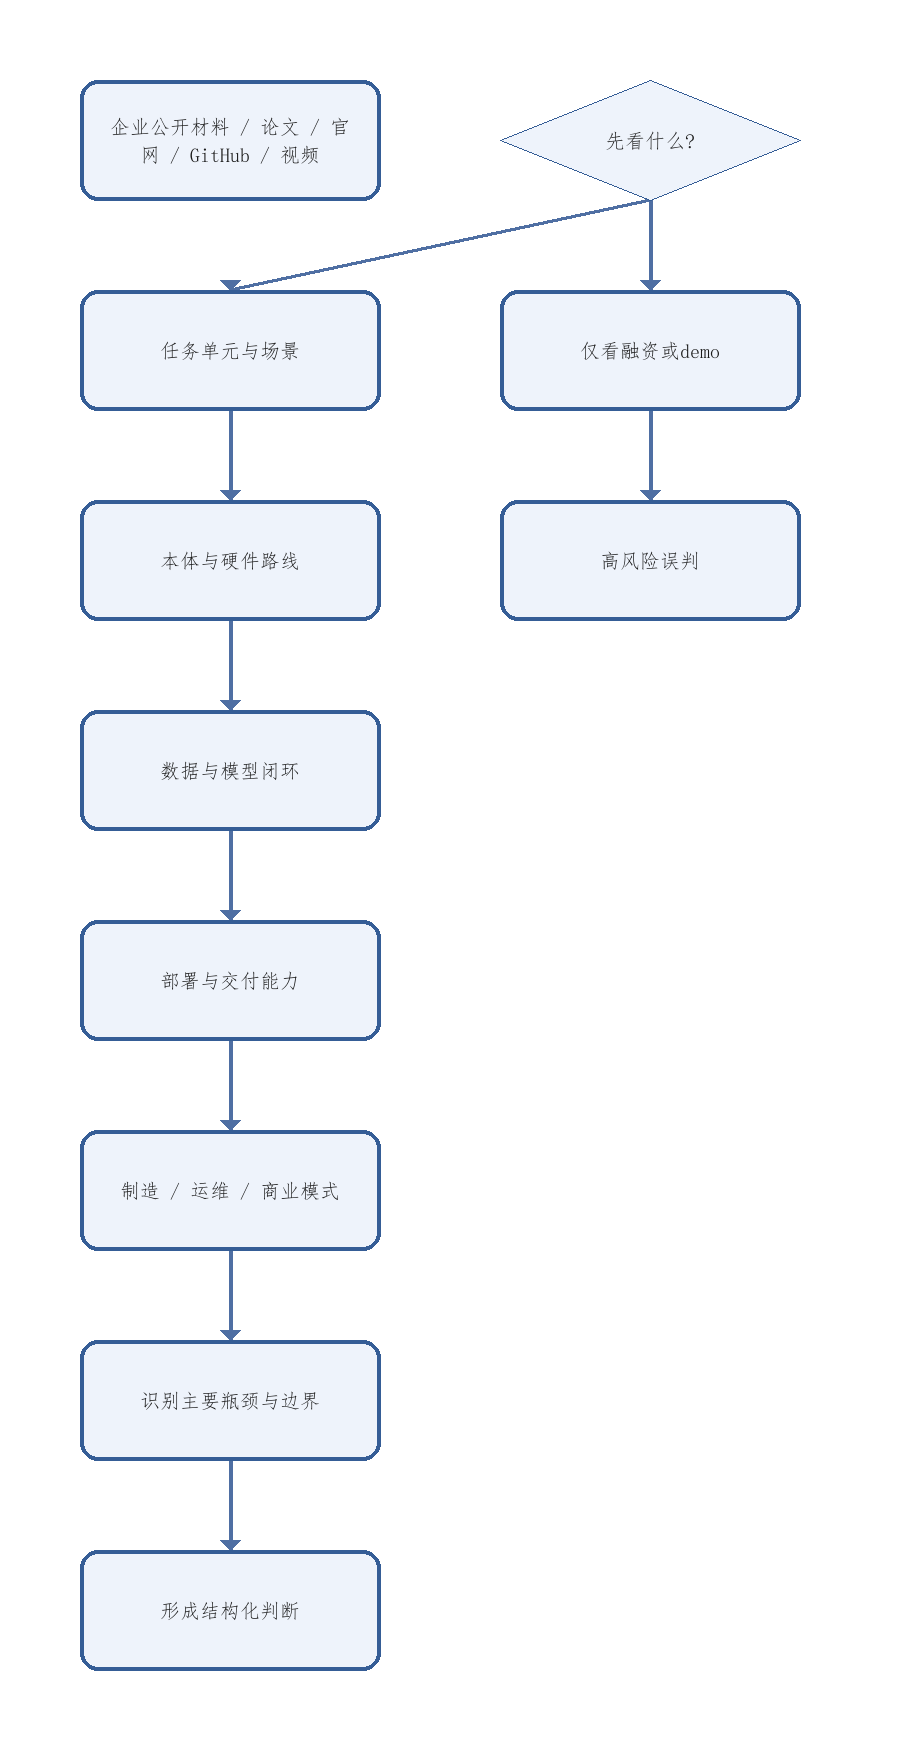
\includegraphics[width=0.9\textwidth,height=0.72\textheight,keepaspectratio]{figures/20-企业分析流程图.png}
\caption{20-企业分析流程图}
\label{fig:20-企业分析流程图}
\end{figure}

\section*{表 20-1 企业统一分析模板}
\addcontentsline{toc}{chapter}{表 20-1 企业统一分析模板}
\markboth{表 20-1 企业统一分析模板}{表 20-1 企业统一分析模板}

\begingroup
\small
\begin{xltabular}{\textwidth}{YYYY}
\toprule
维度 & 核心问题 & 典型证据 & 常见误判 \\
\midrule
\endfirsthead
\toprule
维度 & 核心问题 & 典型证据 & 常见误判 \\
\midrule
\endhead
本体 & 公司控制哪类本体？本体是否是核心护城河？ & 本体规格、负载、续航、自由度、末端执行器 & 只看外形，不看可制造性 \\
模型 & 是做 VLA、技能层、世界模型还是系统集成？ & 论文、博客、技术主页、模型接口 & 把高层语义能力当成完整系统能力 \\
数据 & 是否掌握高质量真机/遥操作/失败回流数据？ & 数据闭环描述、采集系统、数据集合作 & 只看“数据多”，不看数据类型和闭环 \\
部署 & 是否有真实场景、维护体系和恢复机制？ & 客户案例、试点、运维流程 & 把 demo 当部署 \\
制造 & 是否有供应链、量产、成本工程能力？ & 交付节奏、供应链合作、良率信息 & 把原型能力当量产能力 \\
商业模式 & 卖平台、整机、方案还是 RaaS？ & 收费模式、客户类型、合作方式 & 只看融资不看收入结构 \\
主要风险 & 当前最脆弱瓶颈在哪？ & 任务覆盖、成本、可靠性、法规 & 用宏大叙事遮蔽单点瓶颈 \\
\bottomrule
\end{xltabular}
\endgroup

\section*{图表与表格补充}
\addcontentsline{toc}{chapter}{图表与表格补充}
\markboth{图表与表格补充}{图表与表格补充}

这一章末尾之所以需要专门收束为模板、流程图和版本对照样例，是因为它的目标并不是“介绍企业”，而是建立一把可重复使用的分析尺子。没有统一模板时，不同企业极容易被各自的材料口径牵着走；只有先把问题集固定下来，后续企业章节才有可能在相同维度下比较本体、数据、部署、交付和风险。

从版本维护角度看，这组补充材料同样是后续更新工作的关键支点。以后更新企业章节时，最重要的不是重写公司简介，而是沿着同一模板替换事实层、修正判断层，并保留跨版本可对照性。

在当前版本中，\texttt{\detokenize{图 20-1 企业分析流程图}} 已承担“从外部信号进入可交付判断”的流程锚点职责；\texttt{\detokenize{表 20-1 企业统一分析模板}} 则把“本体 / 模型 / 数据 / 部署 / 制造 / 商业模式 / 主要风险”等横向比较维度固定下来。

“同一企业多轮版本更新如何回写判断层”这一问题，本质上要求报告具备跨时间的结构化记忆能力。单靠正文叙述很难稳定维护，因此更适合通过 20-企业季度跟踪表模板 与企业长期跟踪卡来承载。正文负责输出阶段性判断，结构化资产负责记录新增信号、口径变化和判断回调依据，两者结合后，企业研究才不会退化成一次性的公司简介。

为了让这一章真正变成后续维护的工作台，而不是只作为阅读框架存在，建议后续企业更新统一依赖两张表：一张是 20-企业统一分析模板，负责稳定横向比较维度；另一张是 20-企业季度跟踪表模板，负责记录季度新增信号与是否需要回调专题。这样做后，企业章节的更新路径就会从“重写公司简介”转变成“先补信号，再修判断”。

如果需要进一步降低后续维护成本，也可以直接优先使用脚本导出版：20-企业统一分析模板-脚本生成版 与 20-企业季度跟踪表模板-脚本生成版。其底层字段源位于 \path{data/processed/}，便于后续先改结构化字段，再统一导出到正文表格。

作为首批可复用研究资产，后续企业章节还应优先复用以下长期跟踪卡，而不是每次重新从新闻和视频开始：

\begin{enumerate}
\item Google DeepMind 长期跟踪卡
\item NVIDIA 长期跟踪卡
\item Figure 长期跟踪卡
\item 优必选 长期跟踪卡
\end{enumerate}

对于高频变化信号，后续不应直接在长期卡或正文里堆新闻，而应优先记入季度更新日志。当前已建立的样板包括：

\begin{enumerate}
\item 企业季度更新日志模板
\item Google DeepMind 季度更新日志
\item NVIDIA 季度更新日志
\item Figure 季度更新日志
\item 优必选 季度更新日志
\item Agility 季度更新日志
\item Apptronik 季度更新日志
\item 智元 季度更新日志
\item 宇树 季度更新日志
\end{enumerate}

如果后续要把季度信号沉淀到统一结构化表中，则应同步更新 20-企业季度跟踪表模板-脚本生成版 对应的底层 csv，而不是只在正文里补一句“本季度有变化”。
